\documentclass[11pt, a4paper]{report}
\special{papersize=210mm, 297mm}
\usepackage[english]{babel}
\usepackage[utf8x]{inputenc}
\usepackage[left=2.5cm, right=2.5cm, top=2.5cm]{geometry}
\renewcommand{\baselinestretch}{1.4}
\usepackage[toc,page]{appendix}
\pagenumbering{alph}

\usepackage{amsmath}
\usepackage{graphicx}
\usepackage{float}
\graphicspath{{images/} {diagrams/}}
\usepackage{tabularx}
\usepackage{booktabs}

%\usepackage{showframe}
\usepackage{fullpage}

\usepackage{url}
%\usepackage{natbib} % for author-date citation \citep{}, \citet[]
%\usepackage{hyperref}
%\usepackage[nottoc]{tocbibind}
\usepackage{listings}
\usepackage{verbatim}
\usepackage{color}

\definecolor{dkgreen}{rgb}{0,0.6,0}
\definecolor{gray}{rgb}{0.5,0.5,0.5}
\definecolor{mauve}{rgb}{0.58,0,0.82}

\lstset{frame=tb,
	language=java,
	aboveskip=5mm, belowskip=3mm, showstringspaces=false,
	columns=flexible, basicstyle={\small\ttfamily},
	numbers=none, numberstyle=\tiny\color{gray},
	keywordstyle=\color{blue},
	commentstyle=\color{dkgreen},
	stringstyle=\color{mauve},
	breaklines=true,
	breakatwhitespace=true,
	tabsize=3
}


\usepackage{multirow}
\usepackage{array}
\newcolumntype{L}[1]{> {\raggedright\let\newline\\\arraybackslash\hspace{0pt}}m{#1}}
\newcolumntype{C}[1]{>{\centering\let\newline\\\arraybackslash\hspace{0pt}}m{#1}}
\newcolumntype{R}[1]{>{\raggedleft\let\newline\\\arraybackslash\hspace{0pt}}m{#1}}

\pagenumbering{arabic}

\begin{document}
	
	%======================================================================
	
	\begin{titlepage}
		
		\newcommand{\HRule}{\rule{\linewidth}{0.5mm}}
		
		\center
		
		\vspace{-20pt}
		
\includegraphics[width=100pt]{../images/FMI-03.png}\\[1.0cm]
		
		\textsc{\LARGE West University of Timisoara}\\[0.5cm]
		\textsc{\Large Faculty of Mathematics and Computer Science}\\[0.5cm]
		\textsc{\large Study Program: \\Computer Science in English}\\[3cm]
		\textsc{\Huge Master Dissertation}\\[5cm]
		
		\begin{minipage}{0.4\textwidth}
			\begin{flushleft} \large
				\textbf{COORDINATOR:}\\
				Associate Prof. Marc Eduard \textsc{Frîncu}
			\end{flushleft}
		\end{minipage}
		~
		\begin{minipage}{0.4\textwidth}
			\begin{flushright} \large
				\textbf{GRADUATE:} \\
				Maria Minerva \textsc{Vonica}
			\end{flushright}
		\end{minipage}\\[0.5cm]
			
		\vfill
		{\large Timi\c{s}oara \\2021}\\
		\vfill
		
	\end{titlepage}
	
	% =====================================================================
	
	\begin{titlepage}
		
		\newcommand{\HRule}{\rule{\linewidth}{0.5mm}}
		
		\center
		
		\textsc{}\\[.7cm]
		
		\textsc{\LARGE West University of  Timi\c{s}oara}\\[0.5cm]
		\textsc{\Large Faculty of Mathematics and Computer Science}\\[0.5cm]
		\textsc{\large Study Program: \\Computer Science in English}\\[4.5cm]
		
		\textsc{\Huge Master Dissertation}\\[2cm]
		
		{\Huge \bfseries Name}\\[6cm]
		
		\begin{minipage}{0.4\textwidth}
			\begin{flushleft} \large
				\textbf{COORDINATOR:}\\
				Associate Prof. Marc Eduard \textsc{Frîncu}
			\end{flushleft}
		\end{minipage}
		~
		\begin{minipage}{0.4\textwidth}
			\begin{flushright} \large
				\textbf{GRADUATE:} \\
				Maria-Minerva \textsc{Vonica}
			\end{flushright}
		\end{minipage}\\[0.5cm]
		\vfill
		{\large Timi\c{s}oara\\ 2021}\\
		
		\vfill
		
	\end{titlepage}

	% =====================================================================
	
	\chapter{Application}
	\section{Dataset}
	In order to build the dataset, we made use of the freely available data from the Landsat Archive, specifically from collection 1, level 1. This consists of data products generated from Landsat 8 Operational Land Imager/Thermal Infrared Sensor, Landsat 7 Enhanced Thematic Mapper Plus, Landsat 4-5 Thematic Mapper, and Landsat 1-5 Multispectral Scanner instruments \cite{C1L1}. For the purpose of this paper, we will focus only on images collected from the Landsat 8 satellite.
	
	\subsection{Landsat 8}
	\label{seq:landsat8_section}

	For the purpose of this paper, we will use images collected by the Landsat 8 satellite Figure~\ref{fig:landsat_satellite}, which was launched on an Atlas-V rocket from Vandenberg Air Force Base, California on February 11, 2013. Landsat 8 is the most recently launched Landsat satellite and carries the Operational Land Imager (OLI) and the Thermal Infrared Sensor (TIRS) instruments.
	\begin{figure}[h]
		\centering
		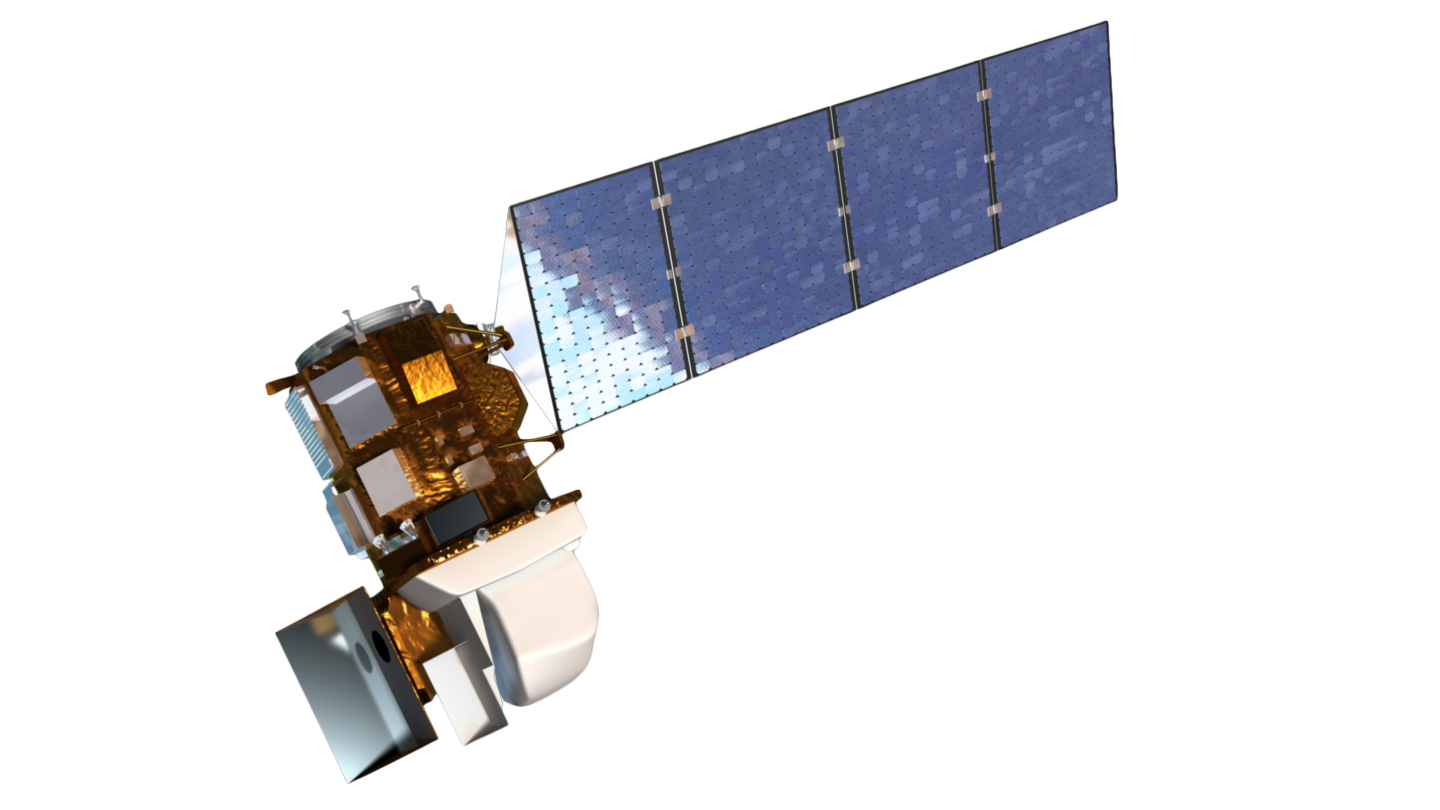
\includegraphics[scale=0.25]{../images/LandsatSatellite.png}
		\caption{Landsat 8 satellite \cite{LANDSATPIC}}
		\label{fig:landsat_satellite}
	\end{figure}
	Landsat 8 orbits the Earth in a sun-synchronous, near-polar orbit, at an altitude of 705 km, inclined at 98.2 degrees, and completes one Earth orbit every 99 minutes.  The satellite has a 16-day repeat cycle with an equatorial crossing time: 10:00 a.m. +/- 15 minutes. It acquires about 740 scenes a day on the Worldwide Reference System-2 (WRS-2) path/row system, with a swath overlap (or sidelap) varying from 7\% at the equator to a maximum of approximately 85\% at extreme latitudes. A Landsat 8 scene size is 185 km x 180 km \cite{LANDSAT}.
	
	\paragraph{Worldwide Reference System-2}
	\label{par:wrs-2}
	
	We will be referring to each scene's location based on its path and row coordinates from the worldwide reference system-2, which is a global notation system for Landsat data. It enables a user to inquire about satellite imagery over any portion of the world by specifying a nominal scene center designated by path and row numbers. The WRS has proven valuable for the cataloguing, referencing, and day-to-day use of imagery transmitted from the Landsat sensors \cite{wrs}. Landsat's trajectory projected on the world map can be seen in Figure~\ref{fig:wrs2}.
	\begin{figure}[h]
		\centering
		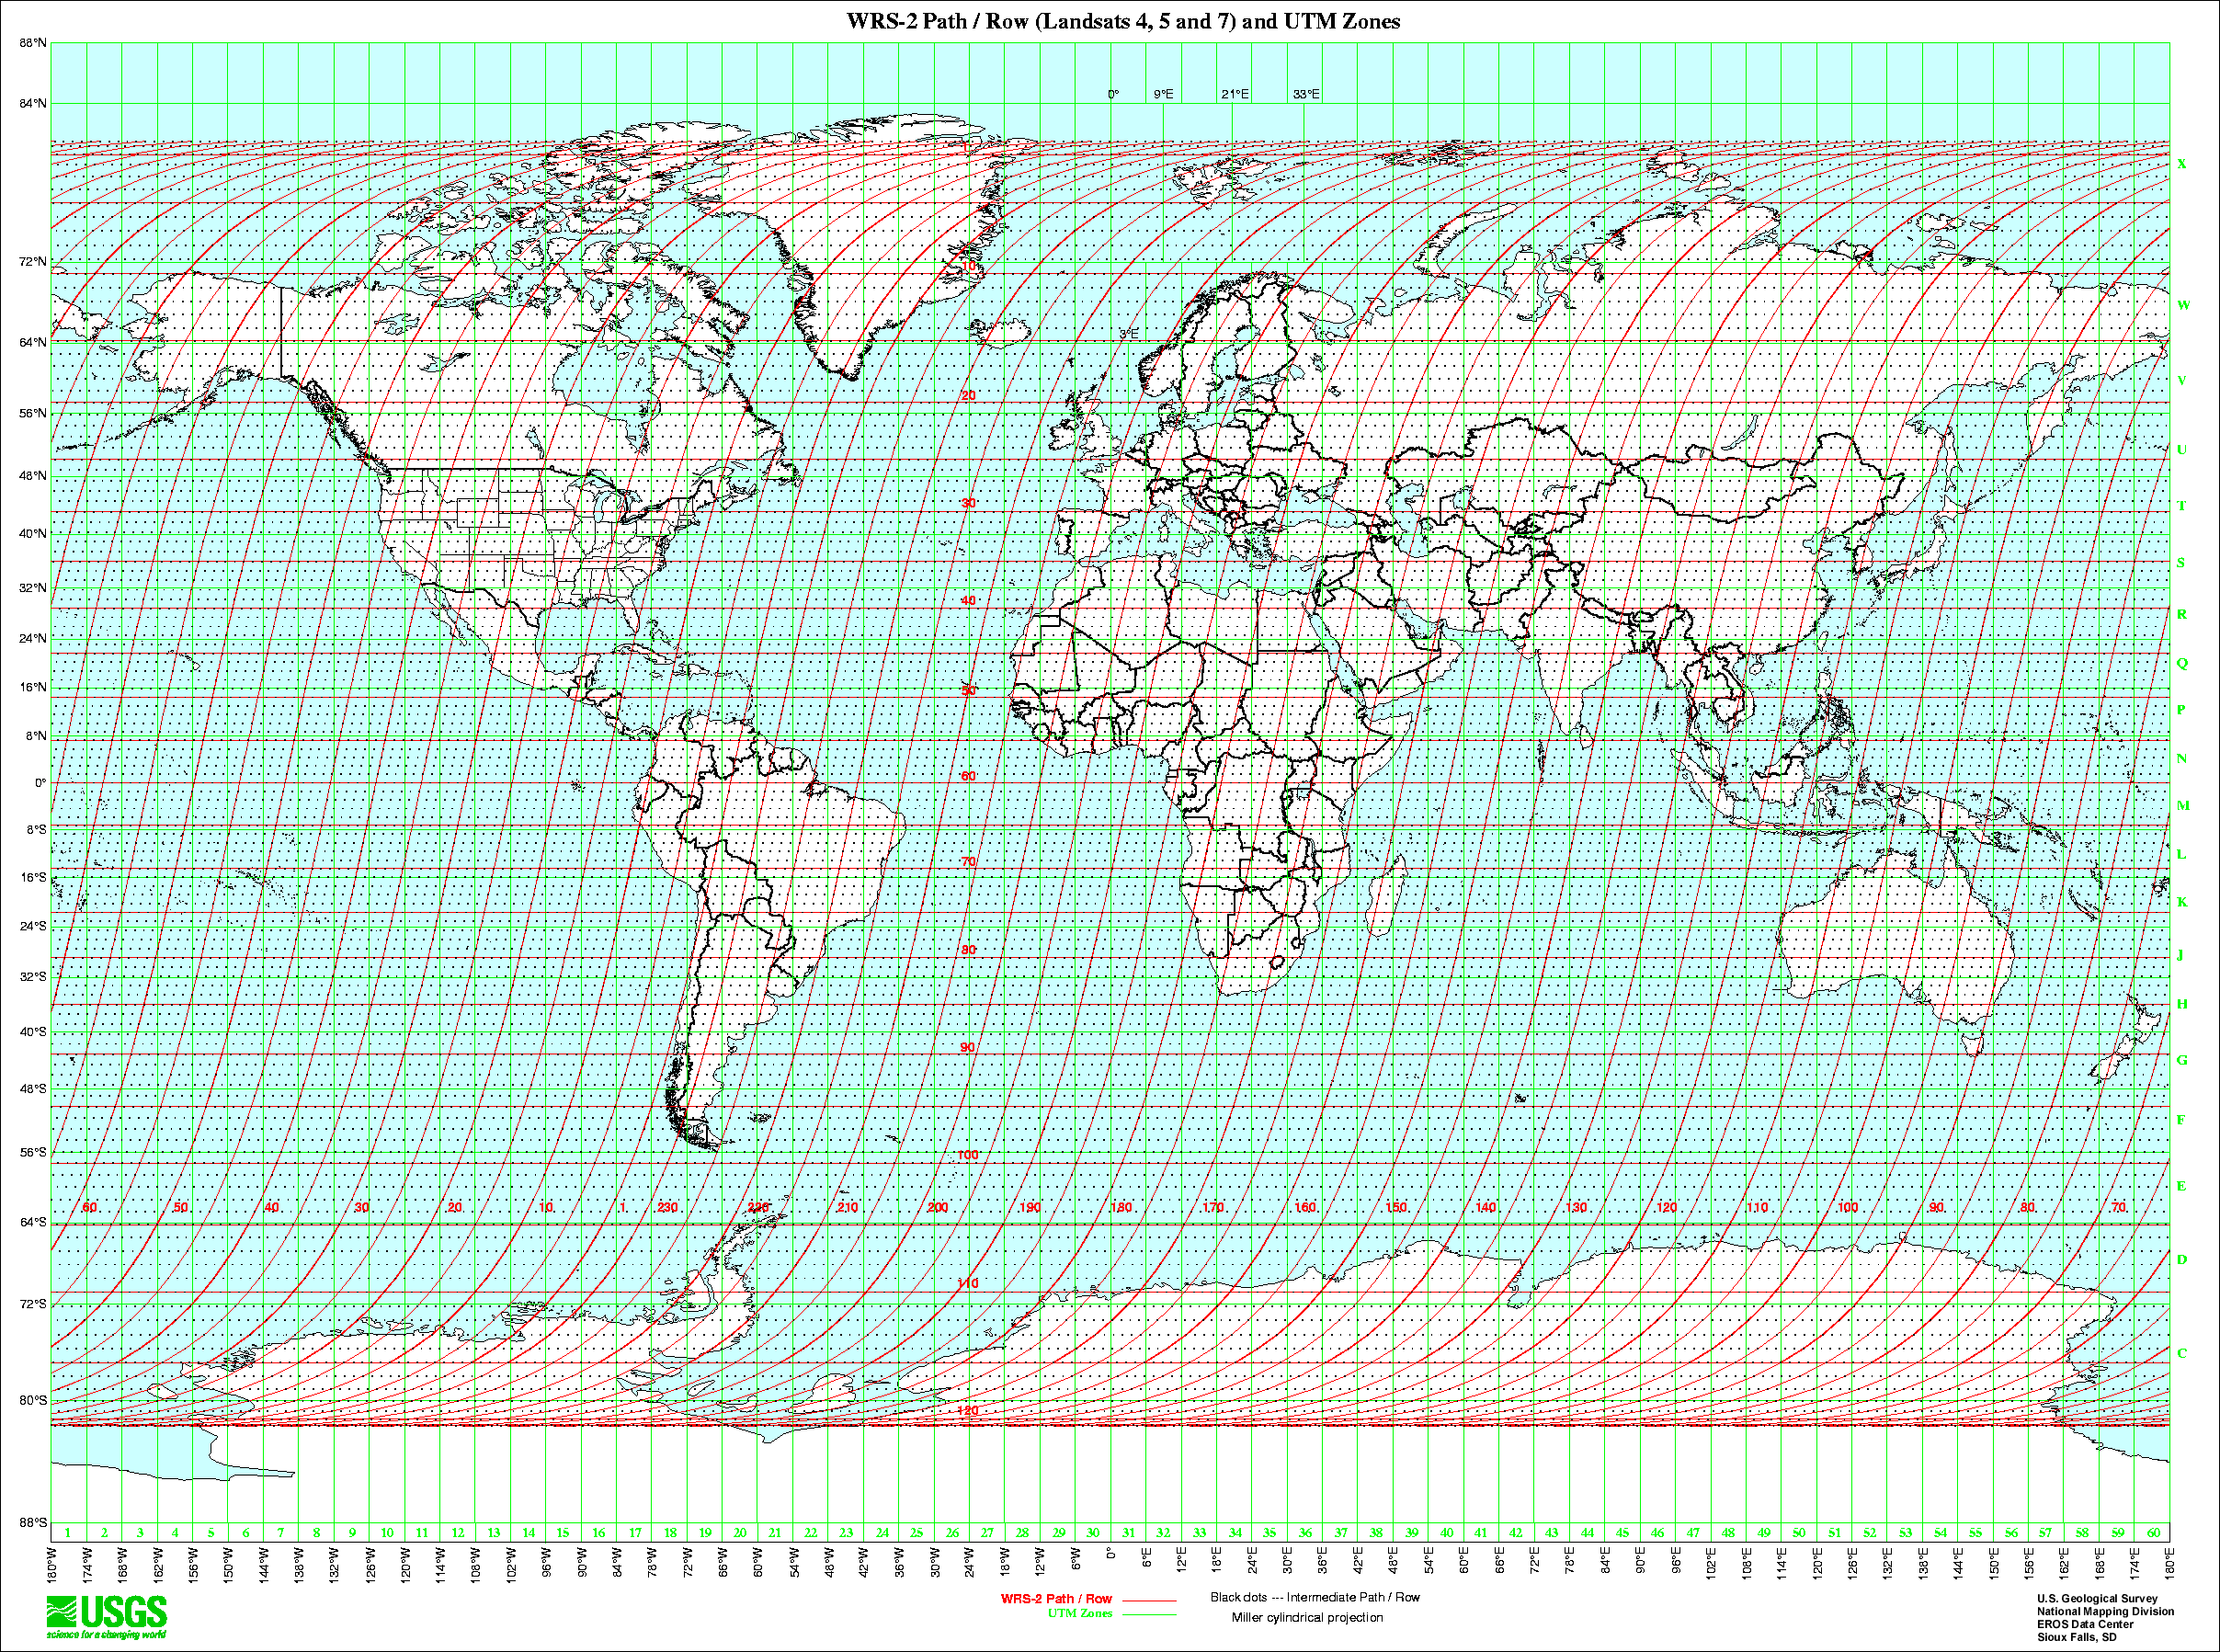
\includegraphics[scale=0.2]{../images/wrs2.png}
		\caption{WRS-2 Path/Row for Landsat \cite{wrs}.}
		\label{fig:wrs2}
	\end{figure}
	
	\subsubsection{Landsat scene naming convention}
	\label{seq:landsat_naming}
	
	Each Landsat scene is named after a well-defined convention in order to easily check information such as the WRS path, row and the date of acquisition. Having access to this information without the need to download the scene itself or the metadata file which holds this information represents a valuable asset, since we can easily filter the data based on the naming convention itself. In the table \ref{table:scene_naming} below we represent what each part of a Landsat scene of the form \textbf{LXS PPPRRR YYYYDDD  GSIVV} means.
	\begin{table} [h]
		\center
		\begin{tabularx}{480pt}{|X|X|}
			\toprule
			\textbf{L} & Landsat \\ [0.2ex]
			\midrule
			\textbf{X} & Sensor \\ [0.2ex]
			\midrule
			\textbf{SS} & Satellite \\ [0.2ex]
			\midrule
			\textbf{PPP} & WRS path \\ [0.2ex]
			\midrule
			\textbf{RRR} & WRS row \\ [0.2ex]
			\midrule
			\textbf{YYYY} & Acquisition year \\ [0.2ex]
			\midrule
			\textbf{DDD} & Julian day of the acquisition year \\ [0.2ex]
			\midrule
			\textbf{GSI} & Ground station identifier \\ [0.2ex]
			\midrule
			\textbf{VV} & Archive version number \\ [0.2ex]
			\midrule
			\midrule
			\bottomrule
		\end{tabularx}
		\caption{Landsat 8 scene naming convention \cite{sn}.}
		\label{table:bands_table}
	\end{table}\label{table:scene_naming}
	
	\subsubsection{Operational Land Imager}
	
	The Operational Land Imager (OLI) is a remote sensing instrument aboard Landsat 8, built by Ball Aerospace \& Technologies. The sensor collects moderate resolution data that is used to monitor changing trends on the surface and evaluate how land usage changes over time. The images and data that OLI has helped collect have practical applications today in agriculture, mapping, and monitoring changes in snow, ice, and water \cite{lolidcp}. 
	The OLI operates in the visible (VIS) and short wave infrared (SWIR) spectral region, having a width of 185 km. It uses nine channels, which range from wavelengths of 443 nm to 2,200 nm. Of these nine channels, eight are multispectral and one is panchromatic. The eight multispectral channels have a 30-meter spatial resolution, and the panchromatic channel has a 15 meters one.
	The OLI generates 9 bands for Landsat as shown in Figure~\ref{fig:L8OLI}.
	\begin{figure}[h]
		\centering
		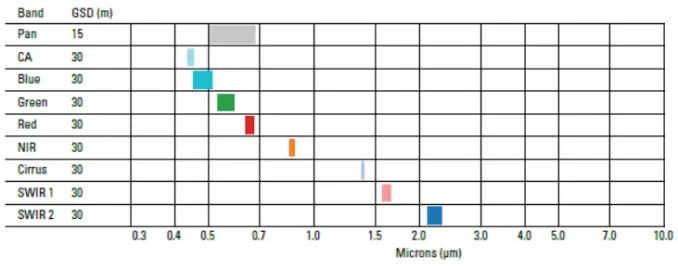
\includegraphics[scale=0.5]{../images/Landsat8-OLI-Bands.png}
		\caption{Landsat 8 OLI generated bands \cite{l8otb}}
		\label{fig:L8OLI}
	\end{figure}
	
	\subsubsection{Thermal Infrared Sensor}
	
	The Thermal Infrared Sensor (TIRS) measures land surface temperature in two thermal bands with a new technology that uses Quantum Well Infrared Photodetectors to detect long wavelengths of light emitted by the Earth whose intensity depends on surface temperature. These wavelengths, called thermal infrared, are well beyond the range of human vision \cite{lgng}.
	The thermal infrared sensor generates 2 bands for Landsat as shown in Figure~\ref{fig:L8TIRS}.
	\begin{figure}[h]
		\centering
		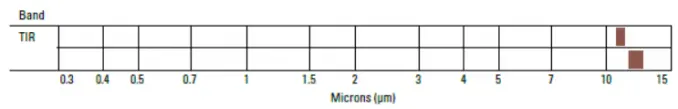
\includegraphics[scale=0.5]{../images/Landsat8-TIRS-Bands.png}
		\caption{Landsat 8 TIRS generated bands \cite{l8otb}}
		\label{fig:L8TIRS}
	\end{figure}
	
	\subsubsection{OLI and TIRS bands}
	
	Landsat 8 acquires data from these sensors in in 11 bands, as following in Table~\ref{table:bands_table}.
	
	\begin{table} [h]
		\center
		\begin{tabularx}{480pt}{|p{0.3\linewidth}|X|X|}
			\toprule
			\textbf{Bands} & \textbf{Wavelength (micrometers)} & \textbf{Resolution (meters)} \\ [0.2ex]
			\midrule
			\midrule
			Band 1 (Coastal aerosol) & 0.43-0.45 & 30 \\ [0.2ex]
			\midrule
			Band 2 (Blue) & 0.45-0.51 & 30 \\ [0.2ex]
			\midrule
			Band 3 (Green) & 0.53-0.59 & 30 \\ [0.2ex]
			\midrule
			Band 4 (Red) & 0.64-0.67 & 30 \\ [0.2ex]
			\hline
			Band 5 (Near Infrared) & 0.85-0.88 & 30 \\ [0.2ex]
			\midrule
			Band 6 (SWIR1) & 1.57-1.65 & 30 \\ [0.2ex]
			\midrule
			Band 7 (SWIR2) & 2.11-2.29 & 30 \\ [0.2ex]
			\midrule
			Band 8 (Panchromatic) & 0.50-0.68 & 15 \\ [0.2ex]
			\midrule
			Band 9 (Cirrus) & 1.36-1.38 & 30 \\ [0.2ex]
			\midrule
			Band 10 (TIR 1) & 10.6-11.19 & 100  \\ [0.2ex]
			\midrule
			Band 11 (TIR 2) & 11.50-12.51 & 100 \\ [0.2ex]
			\midrule
			\bottomrule
		\end{tabularx}
		\caption{Landsat 8-9 Operational Land Imager (OLI) and Thermal Infrared Sensor (TIRS) bands \cite{bands}.}
		\label{table:bands_table}
	\end{table}
	
	\subsection{World Glacier Inventory}
	\label{seq:wgi}
	The World Glacier Inventory (WGI) proves to be a useful resource for building our dataset, since it contains information for over 130,000 glaciers. Inventory parameters include geographic location, area, length, orientation, elevation, and classification. The WGI is based primarily on aerial photographs and maps with most glaciers having one data entry only. Hence, the data set can be viewed as a snapshot of the glacier distribution in the second half of the 20th century. It is based on the original WGI (WGMS 1989) from the World Glacier Monitoring Service \cite{WGI}.  
	There are a number of ways to retrieve data from the inventory:
	\begin{itemize}
		\item download the entire database in a single ASCII text file (wgi\_feb2012.csv);
		\item search by parameter using the Search Inventory interface;
		\item extract regions through the Extract Selected Regions interface.
	\end{itemize}

	The ASCII text file will be used with the purpose to define which are the glaciers to be included in the dataset to be built. An example of how this file looks like can be found in Figure~\ref{fig:WGI_ASCII}.
	
	\begin{figure}[h]
		\centering
		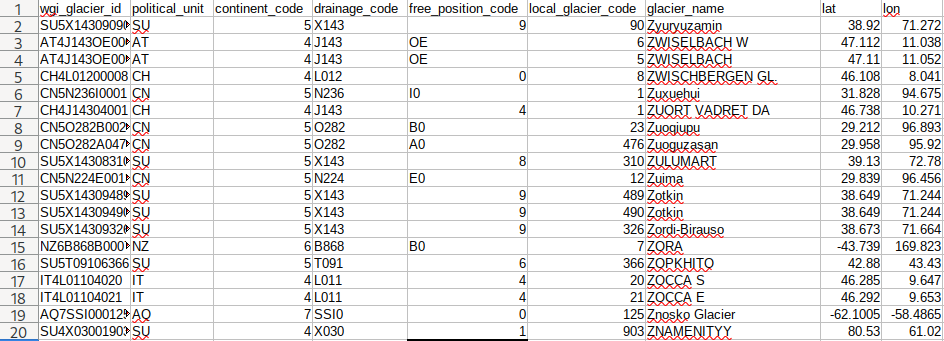
\includegraphics[scale=0.5]{../images/wgi_ASCII_file.png}
		\caption{World glacier inventory ASCII text file, as CSV}
		\label{fig:WGI_ASCII}
	\end{figure}
	
	The \emph{parameters} which will be extracted for the dataset construction are the following:
	\begin{itemize}
		\item \textbf{wgi\_glacier\_id}: unique id representing one glacier (or part of it, if the coverage area is larger);
		\item \textbf{glacier\_name}: name of the glacier (if it has one);
		\item \textbf{lat}: latitude of the glacier;
		\item \textbf{lon}: longitude of the glacier.
	\end{itemize}

	\subsection{Asset Acquisition}	
	
	Since Landsat 8 acquires over 700 scenes per day, this means that there are over two million scenes available for download, either making use of already built user friendly tools or by simply querying for them directly.
	
	\subsubsection{USGS Earth Explorer}
	
	One of the most popular services for satellite imagery downloading is USGS Earth Explorer. This is used for querying and ordering of satellite images, aerial photographs, and cartographic products through the U.S. Geological Survey. The tool is particularly useful when the main focus is to analyse a specific area rather than trying to acquire a large dataset of scenes. One can easily search for assets based on criteria such as world reference system path and row variables, latitude, longitude, cloud coverage, capture date and many others \cite{USGS}.
	
	However, downloading a large set of assets proves to be rather difficult by using this tool alone, since the parameters for each scene need to be manually set. On top of this, the query results have to be picked by hand and then passed for downloading through another application which handles their bulk download. This makes the process of building the dataset rather slow, frustrating and error prone. Such an example can be viewed in Figure~\ref{fig:EarthExplorer}, for the Belvedere glacier (45.942, 7.908).
	
	\begin{figure}[h]
		\centering
		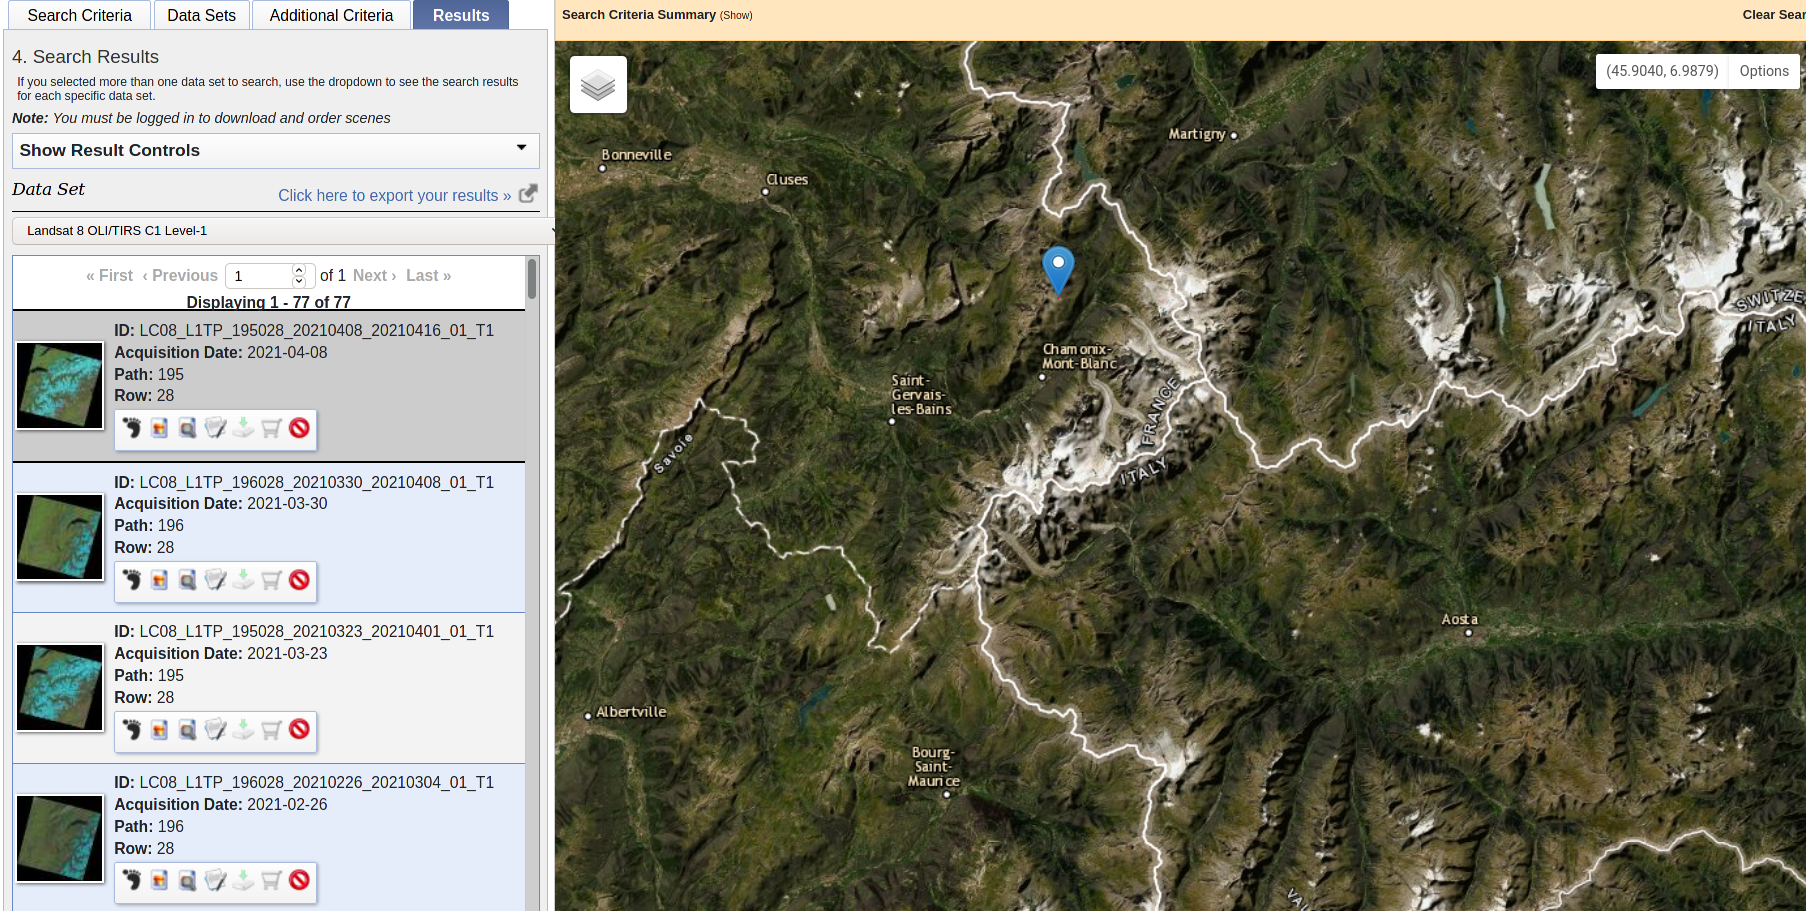
\includegraphics[scale=0.25]{../images/EarthExplorer.png}
		\caption{EarthExplorer}
		\label{fig:EarthExplorer}
	\end{figure}
	
	\subsubsection{SpatioTemporal Asset Catalog API}
	\label{seq:STAC}
	
	In order to fix the problem of excessive manual labour which appeared by using the USGS Earth Explorer, we rather implemented an endpoint of the SpatioTemporal Asset Catalog API, specifically, the following: \textbf{\url{http://nsidc.org/data/glacier_inventory/index.html}} \cite{STAC}. The main idea of searching by using parameters still remains, but instead of manual inputting data for the search data, we rely on using the above-mentioned World Glacier Inventory ASCII text file, since it already has all the required information for each glacier.
	
	By using this method we can pick which glaciers we want to download based on their coordinates and calculate a bounding box representing the area we want to search, required for the STAC API query. Since there might be clouds which could obfuscate the area of interest in the image, we also add a maximum allowed cloud coverage along the bounding box.
	
	The STAC API query also requires a name for the collection of assets we want our queries to be made on, which for us is landsat-8-l1 (Landsat 8 Collection 1, Level 1). Using these three parameters we can now easily acquire a large number of assets with minimal manual labour, as compared to the more user friendly tool provided by USGS.
	
	The downloaded assets will be stored at a user specified disk location and they will be structured as shown in the Figure~\ref{fig:DownloadDirectory}.
	\begin{figure}[h]
		\centering
		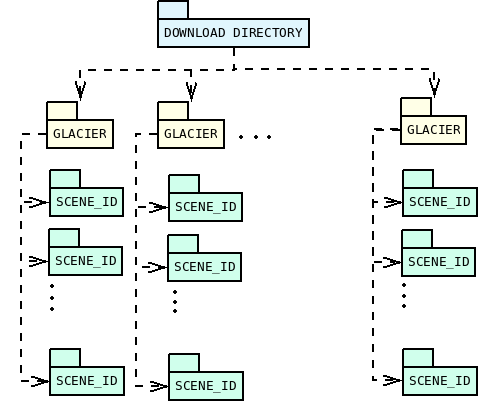
\includegraphics[scale=0.4]{../images/DownloadDirectory.png}
		\caption{Download Directory}
		\label{fig:DownloadDirectory}
	\end{figure}
	
	\subsubsection{Landsat 8 Collection 1, Tier 1}
	
	To support analysis  of the Landsat long-term data record, the Landsat data archive was reorganized  into a formal tiered data collection  structure, which ensures that all Landsat Level 1 products provide a consistent archive of data quality to support time-series analysis and data “stacking”, while controlling continuous improvement of the archive, and access to all data as they are acquired. The implementation of collections ensures consistent and known radiometric and geometric quality through time and across instruments while improving control in the calibration and processing parameters \cite{lc1l1}. By using data from this collection, we ensure that our images are fit for accurate pixel-to-pixel processing.
	
	\section{Dataset entities}
	
	TODO better make this intro...
	We will further describe which are the bands necessary for the image generation and what are their uses. On top of this, we will further explain what is the normalized snow difference index and what is the optical flow used for.
	
	\subsection{Bands}
	
	Each Landsat 8 band is represented by a 16 bit grayscale image with a resolution between 7000 and 10000 pixels, each pixel representing 30 meters. We can conclude, therefore, that one scene covers around 200 and 300 km of Earth. Only the green and SWIR1 bands will be used for the purpose of this thesis and below we will discuss the specifications of each. 
	
	\subsubsection{Band 3 - Green Band}
	
	\begin{table} [h]
		\center
		\begin{tabular} {| l | l |}
			\hline
			\textbf{Wavelength} & {0.53- 0.59 micrometers} \\ [0.2ex]
			\hline
			\textbf{Spacial resolution} & {30 meters} \\ [0.2ex]
			\hline
			\textbf{Resolution} & {between 7000x7000 pixels and 10000x10000 pixels} \\ [0.2ex]
			\hline
			\textbf{Depth} & {16-bit}\\ [0.2ex]
			\hline
			\textbf{Format} & {grayscale}\\ [0.2ex]
			\hline
		\end{tabular}
		\caption{Landsat 8 green band specifications.}
		\label{table:green_table}
	\end{table}
	The green band, alongside with the red and blue ones, fall in the visible spectrum and it is usually used for mapping peak vegetation. Figure~\ref{fig:belvedere_green} is an example of the green band for the Belvedere glacier, specifically taken from scene LC81950282015098LGN01.
	\begin{figure}[h]
		\centering
		
\includegraphics[scale=0.3]{../images/LC81950282015098LGN01_B3.png}
		\caption{Green band of scene LC81950282015098LGN01 from the Belvedere glacier, Italy.}
		\label{fig:belvedere_green}
	\end{figure}
	
	\subsubsection{Band 6 - SWIR1 Band}
	
	\begin{table} [h]
		\center
		\begin{tabular} {| l | l |}
			\hline
			\textbf{Wavelength} & {1.57 - 1.65 micrometers} \\ [0.2ex]
			\hline
			\textbf{Spacial resolution} & {30 meters} \\ [0.2ex]
			\hline
			\textbf{Resolution} & {between 7000x7000 pixels and 10000x10000 pixels} \\ [0.2ex]
			\hline
			\textbf{Depth} & {16-bit}\\ [0.2ex]
			\hline
			\textbf{Format} & {grayscale}\\ [0.2ex]
			\hline
		\end{tabular}
		\caption{Landsat 8 SWIR1 band specifications.}
		\label{table:swir1_table}
	\end{table}
	The shortwave infrared 1 band is particularly useful for enhancing geology objects such as rocks and soils which look similar in other bands \cite{bd}. Alongside this, it also discriminates moisture content of soil and vegetation and penetrates thin clouds \cite{bands}. Figure~\ref{fig:belvedere_swir1} is illustrated below as an example of a SWIR1 band taken from the same scene as the green one above.
	\begin{figure}[h]
		\centering
		
\includegraphics[scale=0.3]{../images/LC81950282015098LGN01_B6.png}
		\caption{SWIR1 band of scene LC81950282015098LGN01 from the Belvedere glacier, Italy.}
		\label{fig:belvedere_swir1}
	\end{figure}
	
	
	\subsubsection{Normalized Snow Difference Index}
	\label{seq:ndsi_functional}
	
	The normalized snow difference index (NDSI) is an index which relates to the presence of snow/ice in a pixel. Snow and ice usually have a very high reflectance in the visible spectrum and very low one in the shortwave infrared one, which is useful for mapping out most types of clouds from the scene \cite{ndsi}. We can therefore use the formula from Equation~\ref{eq:ndsi_formula} in order to highlight the snow and ice pixels from a Landsat 8 image.
	\begin{equation}\label{eq:ndsi_formula}
		NDSI = \frac{green - SWIR1}{green + SWIR1}
	\end{equation}
	By combining the snow reflectance behaviour of snow and ice for each of these bands, we can create a normalized snow difference index image which has values in the range [-1, 1]. We can then apply a threshold on the pixels which states that if the NDSI value for a pixel is larger than 0.0, then that pixel represents snow/ice covered land; similarly, if its value is smaller than 0.0, that pixel represents snow/ice free land \cite{ndsi}, \cite{viirs}, as represented in Equation~\ref{eq:ndsi_threshold}. Of course, this represents the general value for the threshold, but with the increase of its value, we can more accurately differentiate between snow and ice. With larger threshold values we can state that a pixel represents ice covered land rather than just snow fall land \cite{viirs}. We have tried different values for the threshold and came to the conclusion that a value of 0.3 is best suited for our needs.
	\begin{equation}
		\begin{cases}\label{eq:ndsi_threshold}
			\text{snow/ice land} & \text{if } NDSI \geq 0.0\\
			\text{snow-free land}, & \text{NDSI < 0.0}
		\end{cases}
	\end{equation}
	An example of a generated NDSI for the Belvedere glacier, scene LC81950282015098LGN01, can be viewed in Figure~\ref{fig:belvedere_ndsi}.
	\begin{figure}[h]
		\centering
		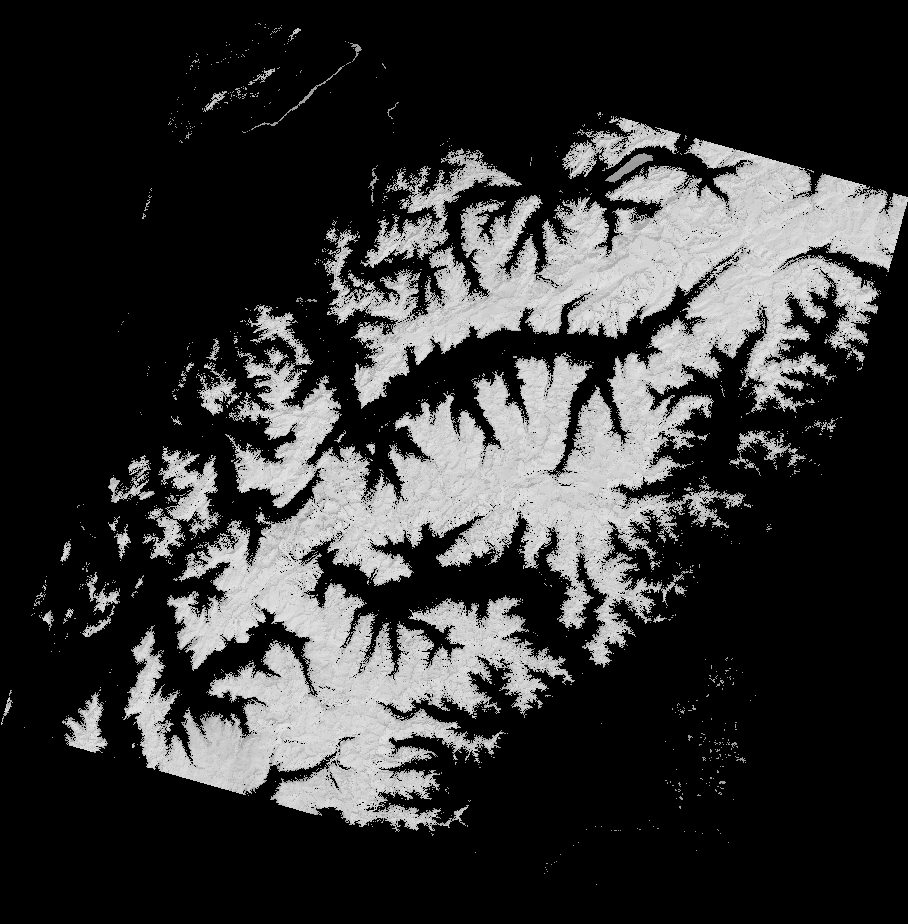
\includegraphics[scale=0.3]{../images/LC81950282015098LGN01_ndsi.png}
		\caption{NDSI of scene LC81950282015098LGN01 from the Belvedere glacier, Italy.}
		\label{fig:belvedere_ndsi}
	\end{figure}

	\section{Alignment}
	\label{seq:alignment_functional}
	Landsat's trajectory orbiting Earth is not fully precise, therefore not all images will be pixel-to-pixel aligned, which is a problem for image processing. Since we want to track each pixel's movement, we must be sure that its coordinates in the image do not change between any two given scenes. Figure~\ref{fig:unaligned} highlights the misalignment from scene between scenes LC81950282013316 and LC81950282013364, as an example.
	\begin{figure}[h]
	\centering
	\begin{minipage}{0.36\textwidth}
		\centering
		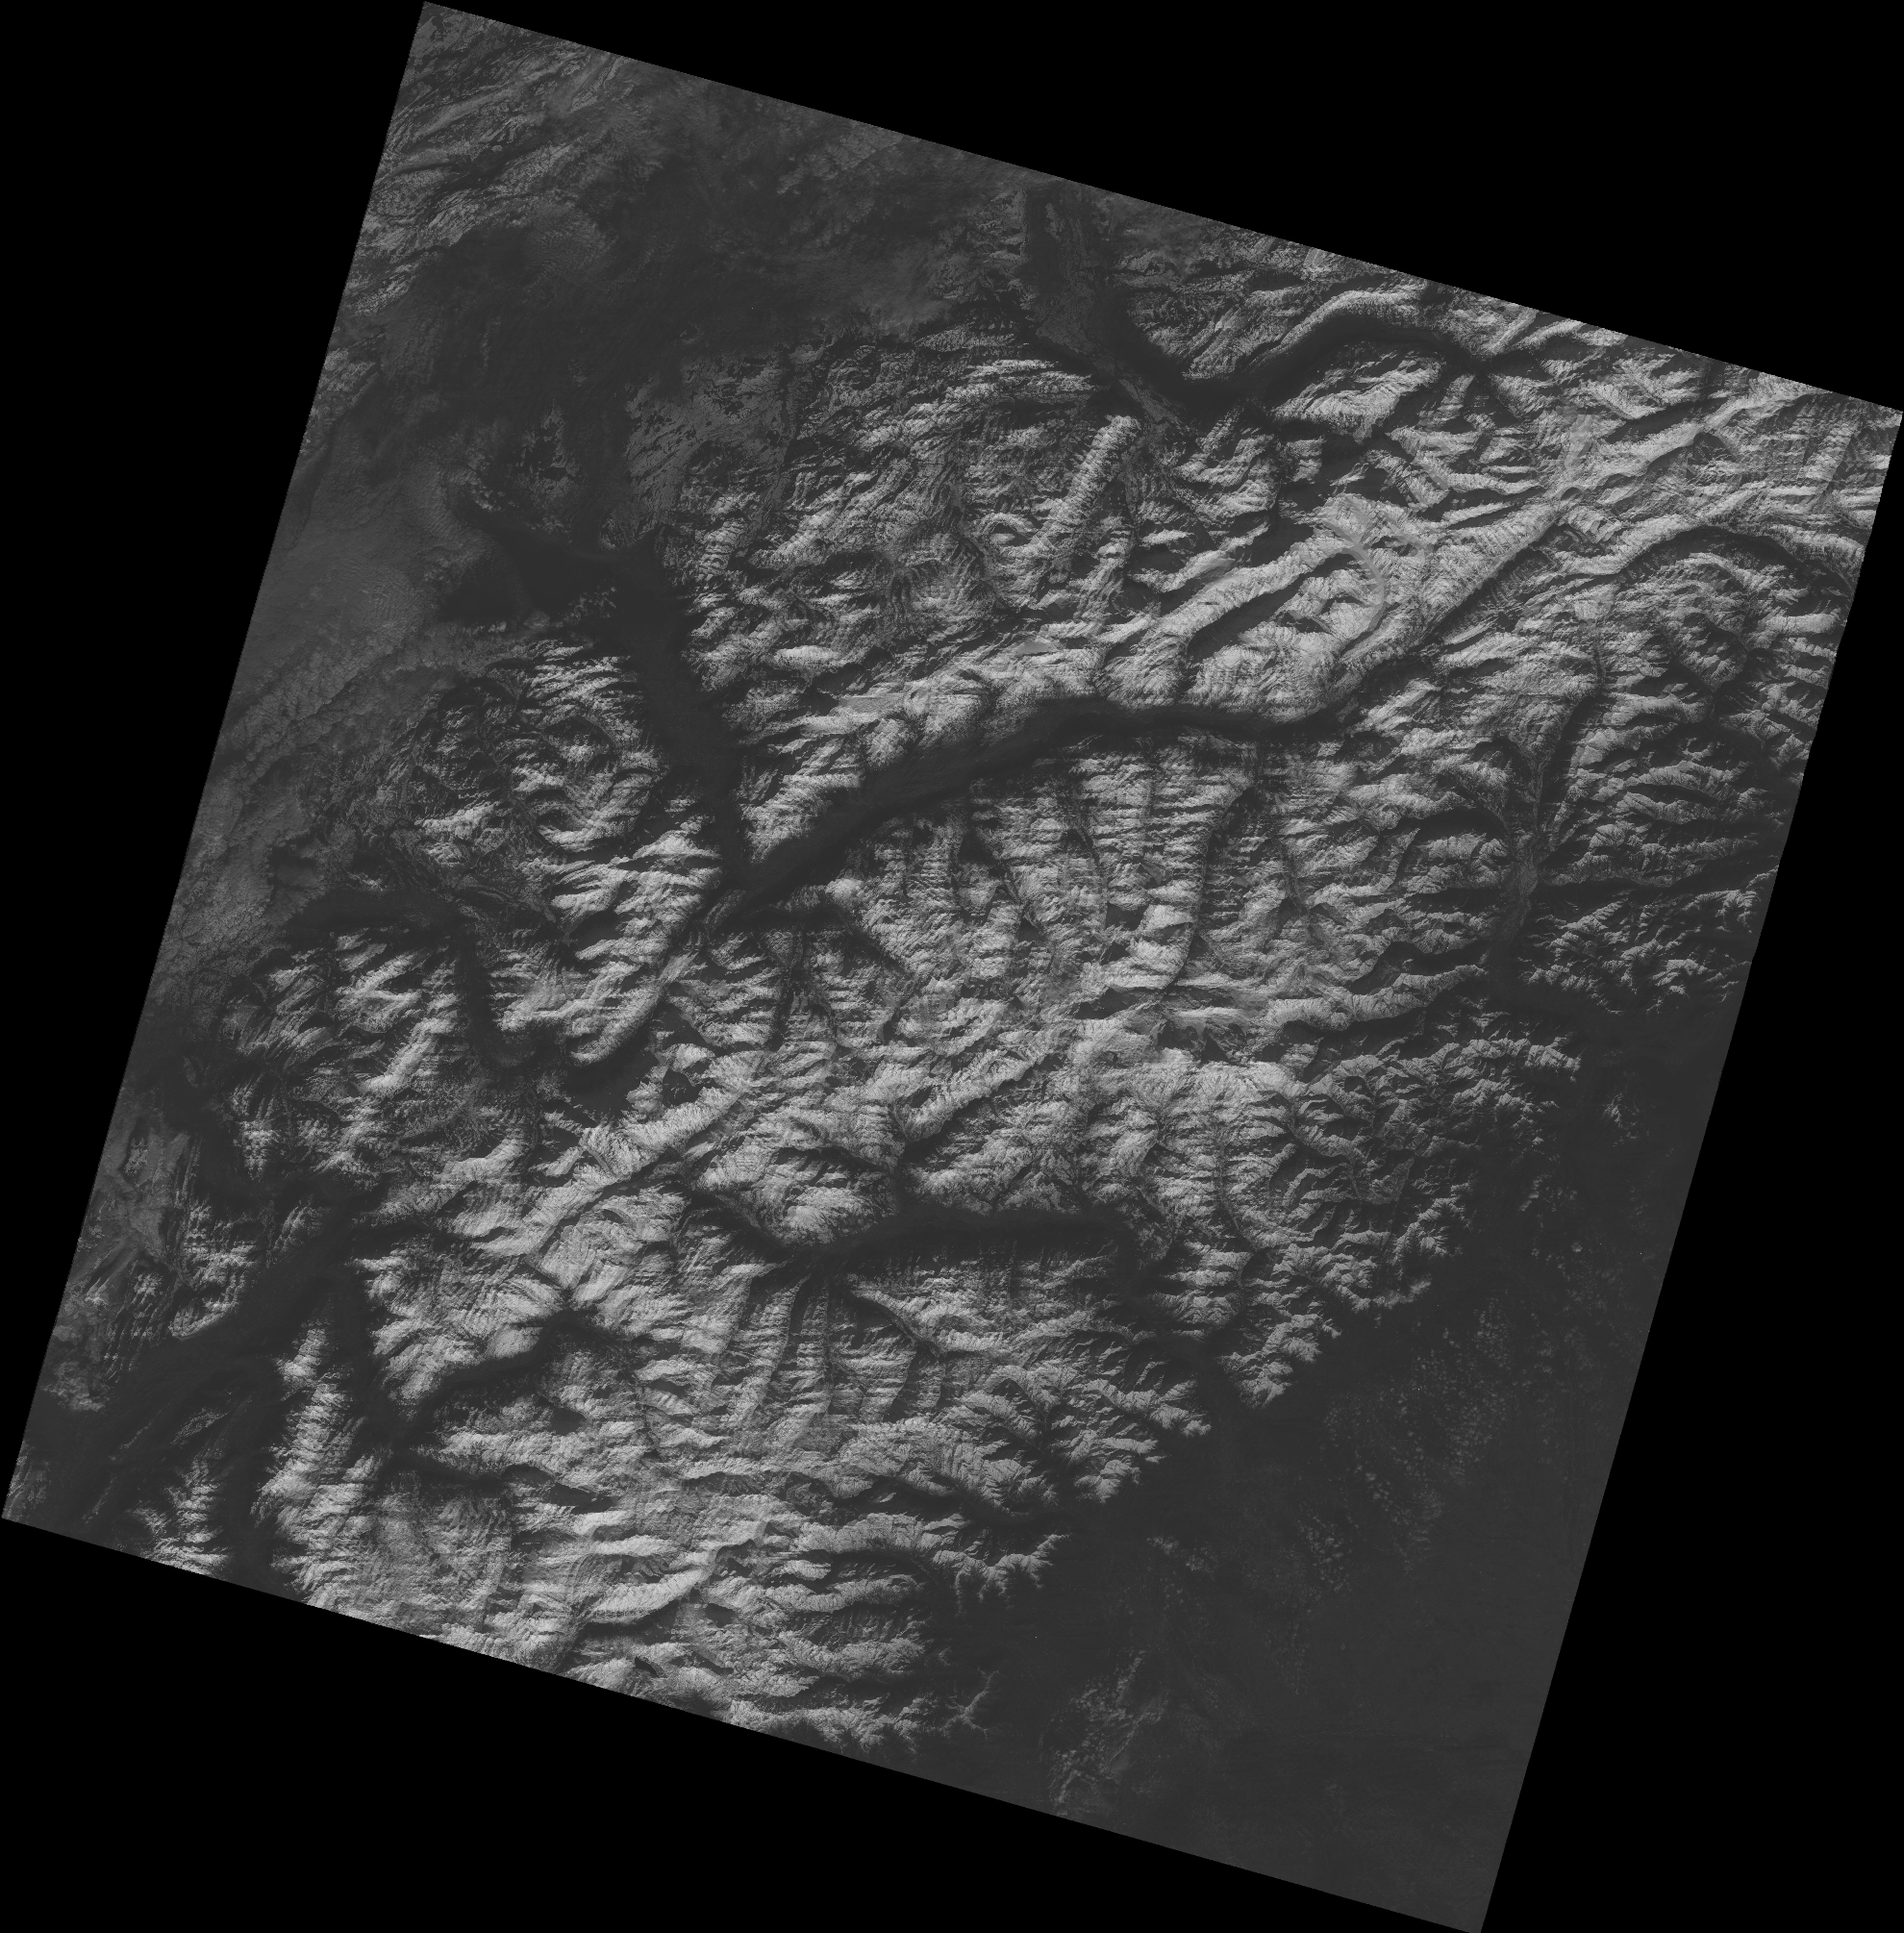
\includegraphics[width=\linewidth]{../images/unaligned.png}
	\end{minipage}
	\begin{minipage}{0.45\textwidth}
		\centering
		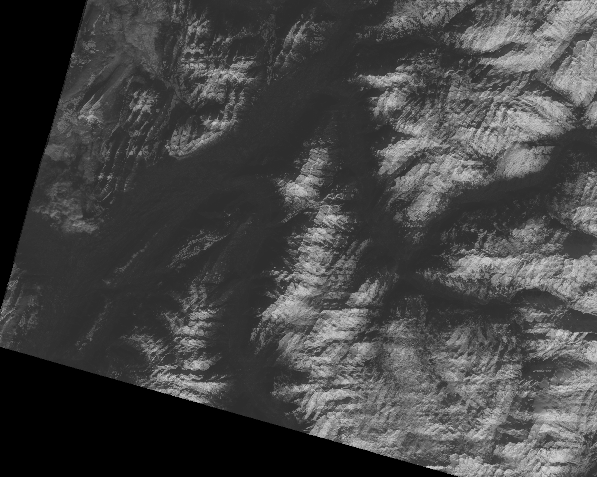
\includegraphics[width=\linewidth]{../images/unaligned_part.png}
	\end{minipage}
	\caption{Overlapped unaligned green band of scene LC81950282013316 and reference LC81950282013364 of the Belvedere glacier (195/028 WRS-2).}
	\label{fig:unaligned}	
	\end{figure}
	Since the bands we work with have a spacial resolution of 30 meters, which means that each pixel in the image represents 30 meters. Even with a misalignment of just 50 pixels we would end up with a 1.5 km difference between two scenes. Tracking pixels through the image without aligning them first would mean that we could never be sure that what we are looking at is indeed the same location. We have used different approaches on alignment which will be described in Section~\ref{seq:alignment_implementation}. Figure~\ref{fig:aligned} highlights the alignment corrected scene from Figure~\ref{fig:unaligned}. 
	\begin{figure}[h]
		\centering
		\begin{minipage}{0.36\textwidth}
			\centering
			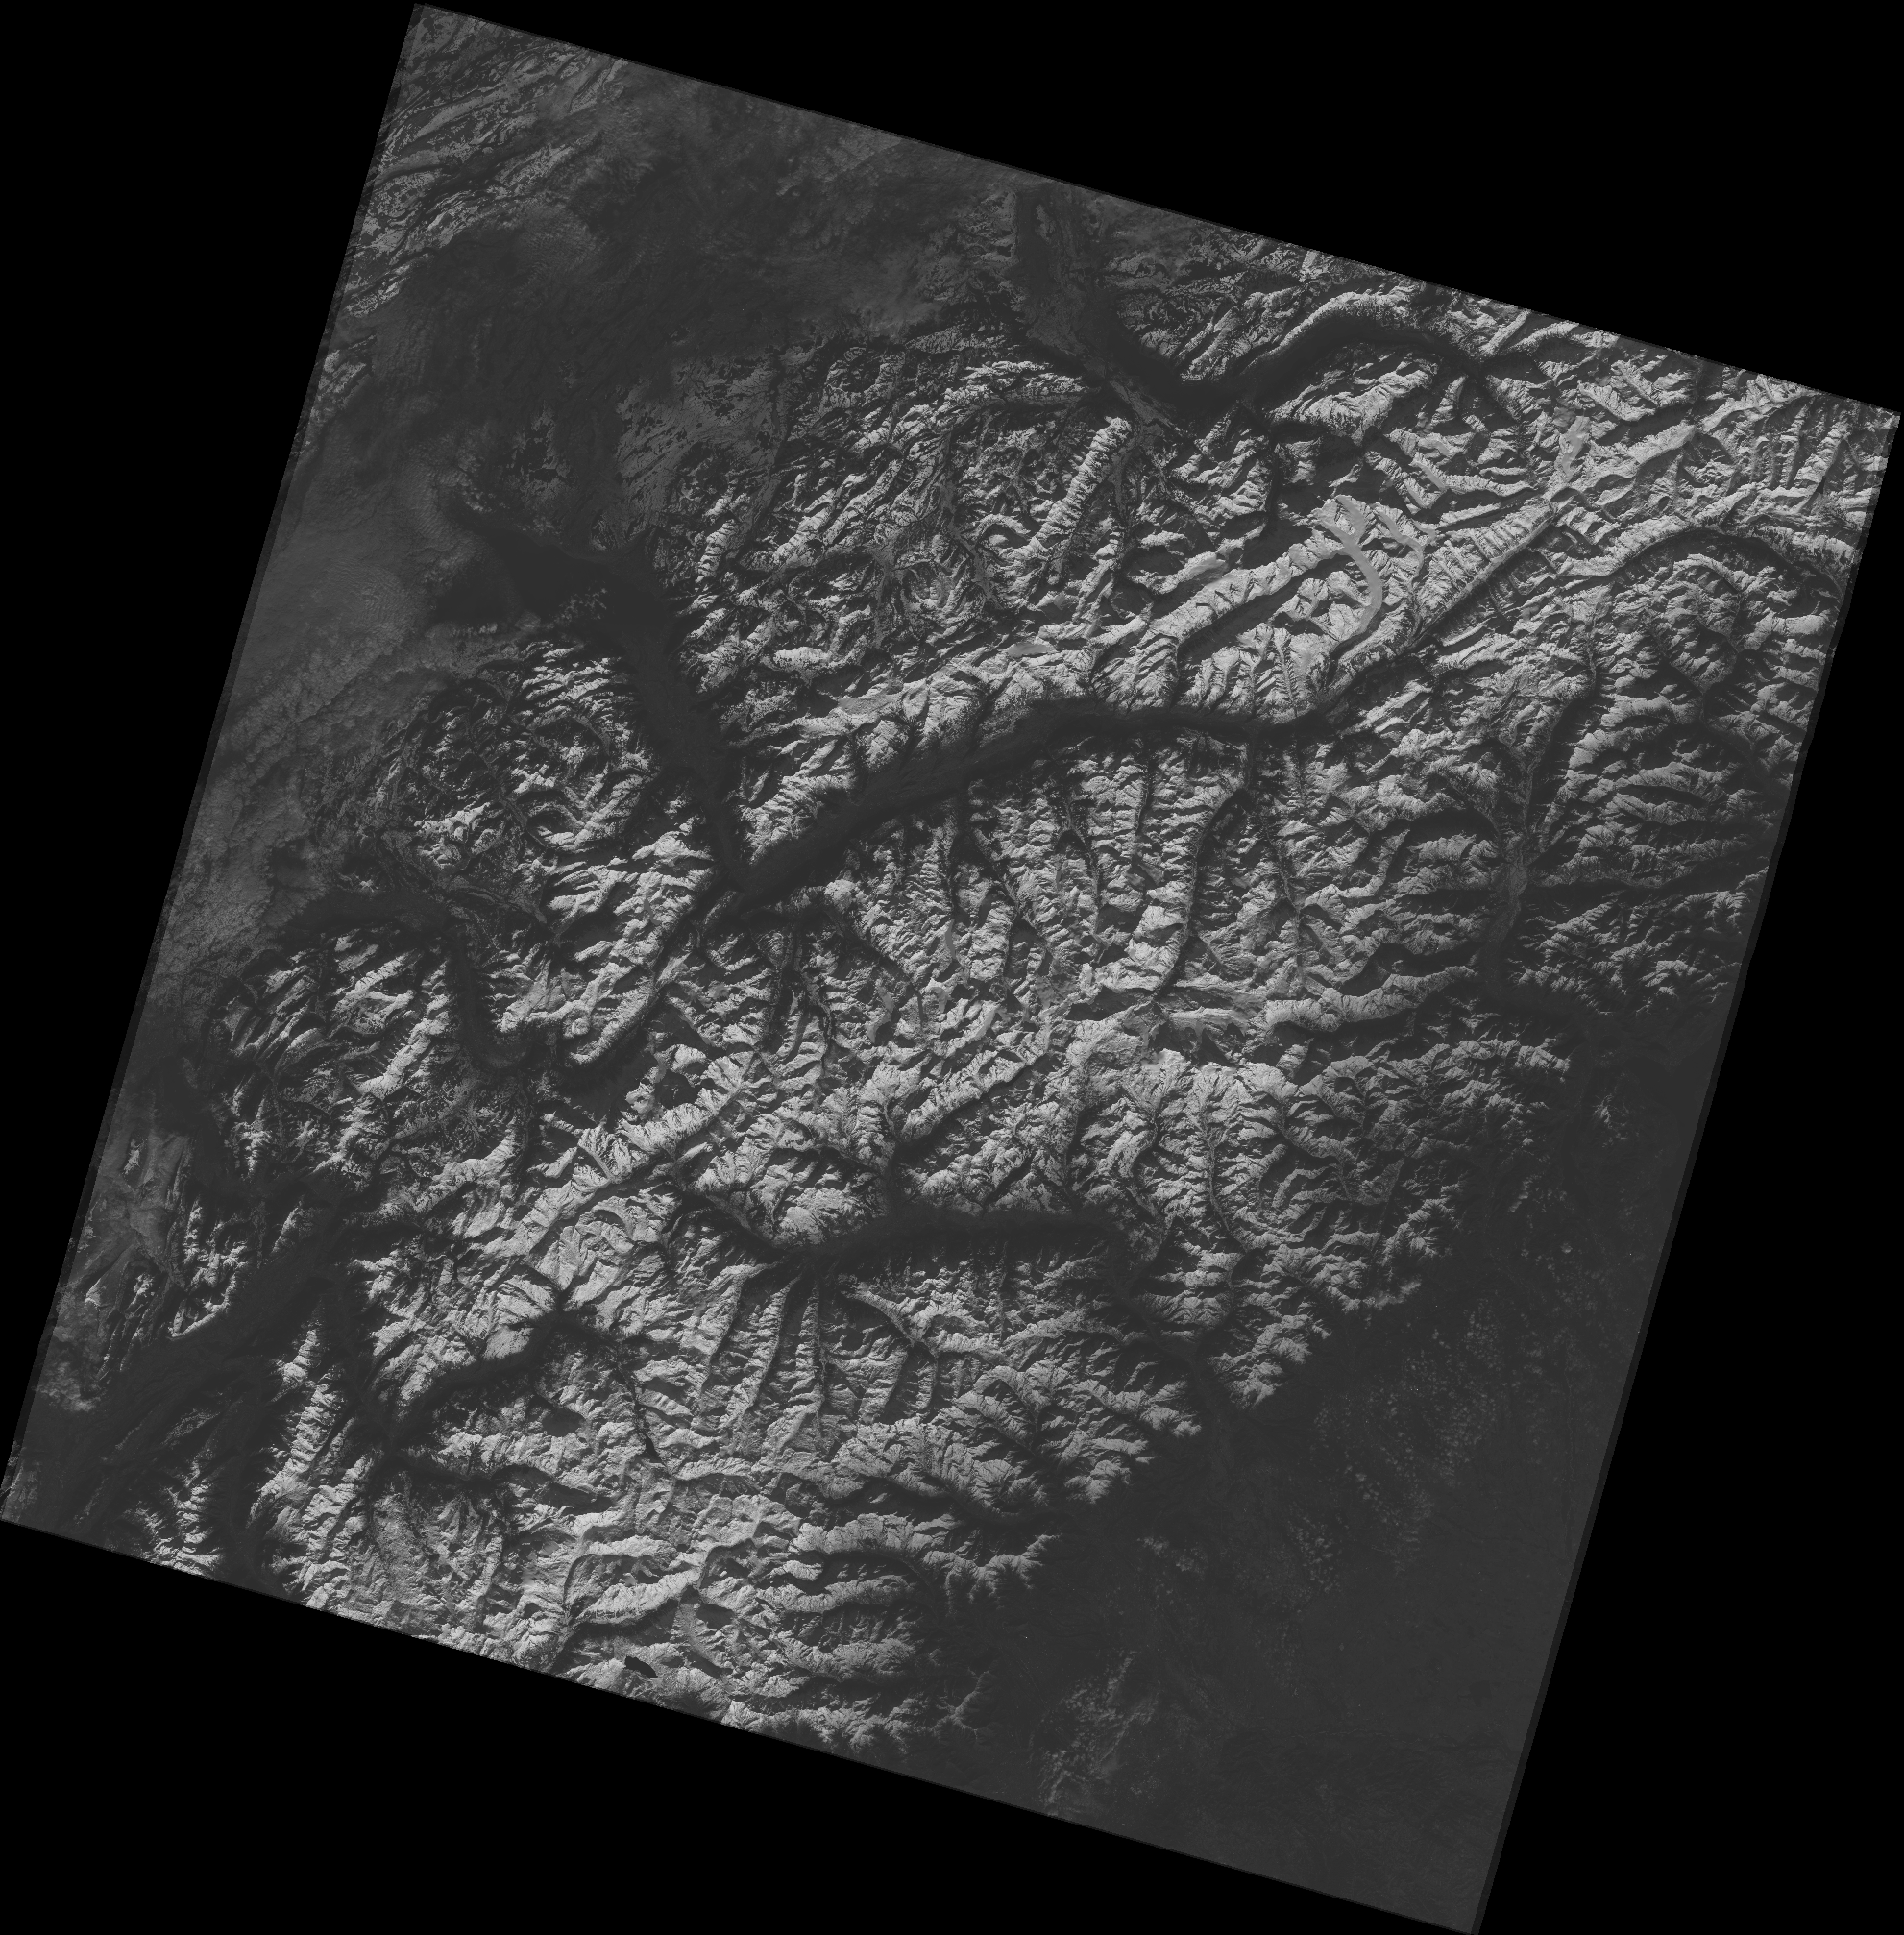
\includegraphics[width=\linewidth]{../images/aligned.png}
		\end{minipage}
		\begin{minipage}{0.45\textwidth}
			\centering
			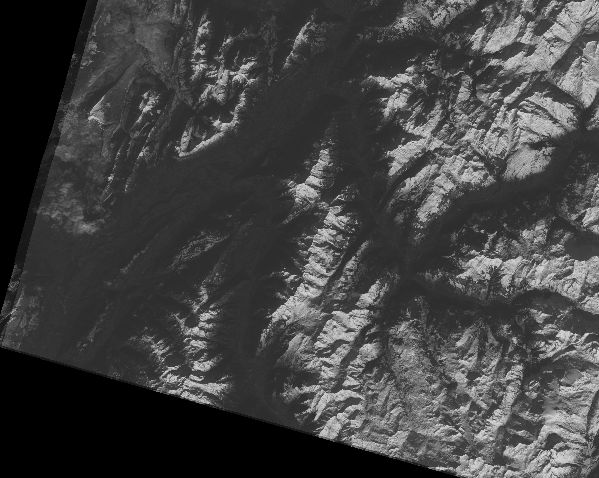
\includegraphics[width=\linewidth]{../images/aligned_part.png}
		\end{minipage}
		\caption{Overlapped aligned green band of scene LC81950282013316 and reference LC81950282013364 of the Belvedere glacier (195/028 WRS-2).}
		\label{fig:aligned}
	\end{figure}

	\subsubsection{NDSI's Motion Matrix}
	\label{seq:ndsi_motion_matrix}
	Since our dataset represents a \textbf{time series of satellite images}, as described in Section~\ref{seq:landsat8_section}, we thought that in order to generate a new image of this series, we could extract the \textbf{motion of each pixel} from one scene to another. This information could then be applied between any two consecutive (date-wise) scenes from the set and we could update a pixel's coordinates based on the value its motion vector and store it in a new image.
	Extracting the motion vectors between two consecutive frames can be achieved by calculating their optical flow. \textbf{Optical flow} is defined as the motion of objects between consecutive frames of sequence, produced by the relative movement between the object and camera. By using computer vision algorithms which calculate the optical flow of two scenes, we could track the motion of melting glaciers across them in order to estimate their current velocity and possibly \textbf{predict their position} in the next frames \cite{opticalflow}.
	\begin{figure}[h]
		\centering
		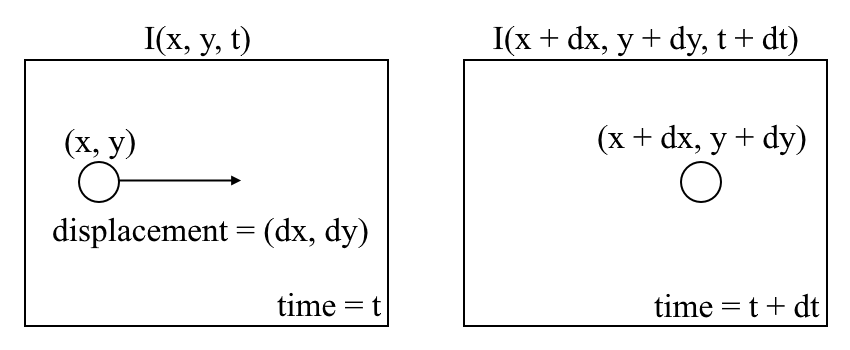
\includegraphics[scale=1.5]{../images/optical_flow_example.png}
		\caption{Optical flow problem visualisation \cite{opticalflow}.}
		\label{fig:optical_flow_example}
	\end{figure}
	
	Figure~\ref{fig:optical_flow_example} emphasizes the problem visually, where we can express an image as a \textbf{function of space}, with the coordinates \textbf{\((x, y)\)}, and \textbf{time} \textbf{\(t\)}. If we take the first image\textbf{ \(I(x, y, t)\)} and we move its pixels by a distance of \textbf{\(dx, dy\)} over a timestamp \textbf{\(dt\)}, we obtain the new image as follows: \textbf{\(I(x + dx, y + dy, t + dt)\)} \cite{orb}.
	
	There are multiple types of optical flow algorithms, but for the purpose of our thesis, we have chosen the \textbf{dense optical flow} one, specifically \textbf{Gunnar Farneback's}. Even if dense implementations have higher cost we chose to make this trade mainly because it calculates the motion for each pixel of the frame and it also has a higher accuracy \cite{orb} compared to methods such as Lucas-Kanade (sparse) \cite{lukas}.
	
	By calculating the optical flow of two consecutive scenes, we construct a matrix which holds the vectors of motion for each pixel, as following.

	\subsubsection{Motion Generated NDSI}
	\label{seq:motion_generated_gui}
	TODO
	\section{Graphical User Interface}
	\label{seq:gui}
	\subsection{Search and Download}
	\label{seq:search_download})

	\chapter{Design and Implementation}
	\label{cha:design_and_implementation}
	
	The design of the application will be discussed while focusing on two different aspects:
	\begin{itemize}
		\item \textbf{search and download}
		\item \textbf{processing}
	\end{itemize}
	The first section is optional and can be run independently from the processing, since the user can have an already created database of images. However, we have focused on simplifying the process of satellite imagery downloading as described in \ref{seq:STAC} through using the sat-search library as a helper for searching and downloading assets. More information on querying can be found in \ref{seq:sd_implementation}. 
	Given an existing set of data, the next step is to pass the root folder which contains the glacier directories to the processing unit, also designed as a plug-in mechanism which will trigger the graphical user interface to pop up and allow for the processing options to appear. More information on this section can be found at \ref{seq:processing}. From there, one can start processing by simply making use of the predefined buttons described in \ref{seq:gui}.
	
	\section{Search and Download}
	
	Searching as well as downloading have been implemented on top of the sat-search library and it is used directly from the command line interface by running the script described in Section~\ref{seq:search_download}.
	As an input we will be using a CSV file which will have the form as described in Section~\ref{seq:wgi}. Mainly we will need just four attributes to be specified for each desired glacier in order to create a query for searching, as follows: \textit{wgi\_glacier\_id, glacier\_name, lat and lon}.
	The CSV file will be intercepted by the \textbf{Download } class and sent for processing row by row (glacier by glacier) to the \textbf{GlacierFactory} class. This one is responsible for parsing each row of the input CSV file and transforming the information in \textbf{Glacier} objects, which will be passed back to the \textbf{Download} class.
	Using the newly created Glacier object we can construct its \textbf{search query} by calculating its bounding box, specifying the asset collection from which we request data and setting other parameters (maximum allowed cloud coverage, in our case). Listing~\ref{lst:query} represents an example of querying for glacier Belvedere, with the following parameters set in the CSV file: \textit{"IT4L01211009","BELVEDERE","45.942","7.908"}.
	\begin{lstlisting}[caption={Search query created by sat-search},label={lst:query},language=Bash]
		{"page": 1, "limit": 170, "bbox": [7.907990000000001, 45.94199, 7.90801, 45.94201], "query": {"eo:cloud_cover": {"lt": 10}}, "collection": "landsat-8-l1"}
	\end{lstlisting}
	The result of each glacier query will be automatically saved in a \textbf{JSON file} which is used as a data buffer between the search and download. The downloader takes each JSON file generated by the search engine and sends the command for getting that asset.
	The technical specifications of the Download, GlacierFactory and Glacier classes can be found in Figure~\ref{fig:sd_diagram}.
	\label{seq:sd_implementation}
	\begin{figure}[h]
		\centering
		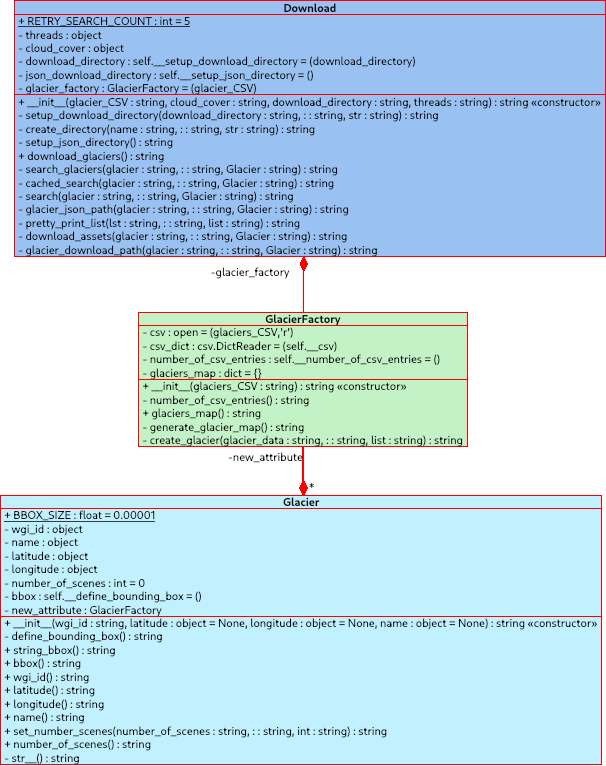
\includegraphics[scale=0.23]{../images/sd_diagram.png}
		\caption{Technical specifications of Download, GlacierFactory and Glacier classes.}
		\label{fig:sd_diagram}
	\end{figure}
	\paragraph{Data corruption verification}
	Both the searching and downloading functions are executed concurrently, since they are \textbf{time intensive} tasks. Each band has around 60 MB, which would make one scene approximately 360 MB. For the Belvedere glaciers, we found 78 scenes with a cloud coverage of 10\%. This means that the size of the entire glacier data will be around 28 GB. Given that one asset's size is quite large, it takes a lot of time to finish the download. In this time, even a small connection interruption might result in corrupted data files, which would interfere with processing. Therefore, we implemented an \textbf{extra security measure} in the sat-stac library which verifies whether a file with the same name already exists at the download location. If it does, its size will be compared to the size taken from the STAC-API servers. In case the two file sizes don't match, it means that the file got corrupted during download and it will be downloaded again. If the sizes match, the downloader will skip the file and continue when it finds one requested file which was not yet found on the disk, such that we do not end up unnecessarily overwriting the already existing files in case of failure.
	
	\section{Processing}
	\label{seq:processing}
	Processing can be viewed as four different entities, as following:
	\begin{itemize}
		\item Image alignment;
		\item Normalized snow difference index;
		\item NDSI's motion matrix;
		\item Motion generated NDSI.
	\end{itemize}
	Before generating any images, we first need to make sure that the pixels between any two scenes are not misaligned. The details of the alignment process are described in Section~\ref{seq:alignment_implementation}. After we ensure that out images are fit, we move on to creating the normalized snow difference index image in order to enhance the ice through a set threshold (see Section~\ref{seq:ndsi_implementation}). We then create the matrix of pixel motions calculated between two consecutive (date-wise) scenes, process described in Section~\ref{seq:motion_matrix_implementation}. Based on the information of where each pixel has moved between two consecutive images, we can then create our future NDSI image by applying the motion vectors on each pixel from a scene. More details on the design and implementation of this part can be found in Section~\ref{seq:motion_ndsi_implementation}.
	The normalized snow difference index image will be computed for each scene as described in Section~\ref{seq:ndsi_functional}.
	
	%========================================================================================
	
	\subsection{Alignment}
	\label{seq:alignment_implementation}
	
	In order to keep a high level of abstraction, we have split each scene into aligned and unaligned: Scene and AlignedScene objects. These and their children are created when crawling through the glaciers directory, specifically for each region of interest. However, aligning all the images when crawling would result into a lot of idle time for the user when starting the application and it would not be overall feasible to do so. Therefore, a scene is aligned only when it is specifically being selected in the graphical user interface (or when another entity needs it, such as optical flow and image generation). By doing this, we ensure that there is no unnecessary extra waiting time for each scene that we have when powering up the interface.
	As for the actual alignment, we have used an algorithm which \textbf{collects features} from each band of a scene and tries to match them with a given reference one's features. The obtained \textbf{matches} can be then used to create an \textbf{affine transformation matrix} which specifies by how much did the current image \textbf{rotated and translated} in comparison to its reference. The affine transformation matrix will be then applied to the current image by a \textbf{warping} algorithm with the goal of ensuring as much as possible that there is no misalignment between any pixel of two different images from the same time series. Section~\ref{seq:alignment_algorithm} describes more technically how we built this and what were the computer vision algorithms used for that matter.
	
	\subsubsection{Alignment algorithms}
	\label{seq:alignment_algorithm}
	
	As we have seen in Section~\ref{seq:landsat8_section}, the Landsat 8 satellite does not have a perfect trajectory, which results into misaligned images. These changes are not obvious to the naked eye from scene to scene, but overlapping two scenes highlights this problem, as we can see in Figure~\ref{fig:unaligned_scene_big}. Even so the scenes are almost similar, which means that aligning them does not prove to be very hard and it is done by using a strong \textbf{keypoint detection algorithm} which in our case detects edges formed by mountains and other geographical features present in the scenes. The \textbf{computer vision algorithms} used for this are \textbf{ORB (Oriented FAST and Rotated BRIEF)}, \textbf{Harris Corner Detector} and \textbf{RANSAC (Random Sample Consensus)} and they are applied on the raw 16bit grayscale image.
	
	\textbf{ORB} represents a fusion between the features from accelerated segment test (\textbf{FAST}) keypoint detector and binary robust independent elementary features (\textbf{BRIEF}) descriptor. The FAST detector finds keypoints in the image and uses Harris corner measure to select the a number of top points from the list (25\%, in our case) \cite{orb}. In order to use the detector we must first normalize and downsample the 16bit raw image to 8 bit, as it is required by ORB. Each keypoint is then represented by a circle of 16 pixels. The descriptors must then identify these keypoints and pair with each other.
	We compute for each scene its \textbf{keypoints and descriptors} taken from \textbf{each band}, in order to increase the precision of alignment later on. Also, since we are working with satellite imagery there might be cases when the algorithm only finds keypoints in a small part of the image, resulting in erroneous distortion. \textbf{Splitting} the image into multiple boxes and applying the orb detect algorithm on each separate part of the image proved to solve this problem and create much better results. 
	
	After ensuring that we have good enough keypoints we will be aligning each scene with its reference by simply comparing the keypoint-descriptor pairs between the two scenes and checking which are equal. If two pairs are found to be equal, it means that the algorithm has found the same feature in both images and can calculate by how much it \textbf{rotated and shifted}. However, not all of these matches represent good results in our case, since the trajectory Landsat 8 can vary. We have found that selecting only \textbf{5000 keypoints} in the \textbf{top 25\% matches} from the total yielded in the better results overall. We then set the \textbf{maximum allowed shifting euclidean distance} between any two pixels to be at most 200, so 6km on the map, therefore getting rid of outlier matches based on the distance.
	The \textbf{matches} from the reference and image to be aligned will be used alongside the \textbf{Random Sample Consensus (RANSAC)} algorithm in order to create the \textbf{affine transformation matrix} using the cv2 library. RANSAC, proposed by Fischler and Bolles \cite{ransac}, is a general parameter estimation approach designed to handle a large proportion of outliers in the input data \cite{ransac2}. After we have the transformation matrix, we can \textbf{warp} it on the image to be aligned in order to get the result. Figure~\ref{fig:alignment_diagram} contains the technical details of each class which takes part into the alignment process.
	\begin{figure}[h]
		\centering
		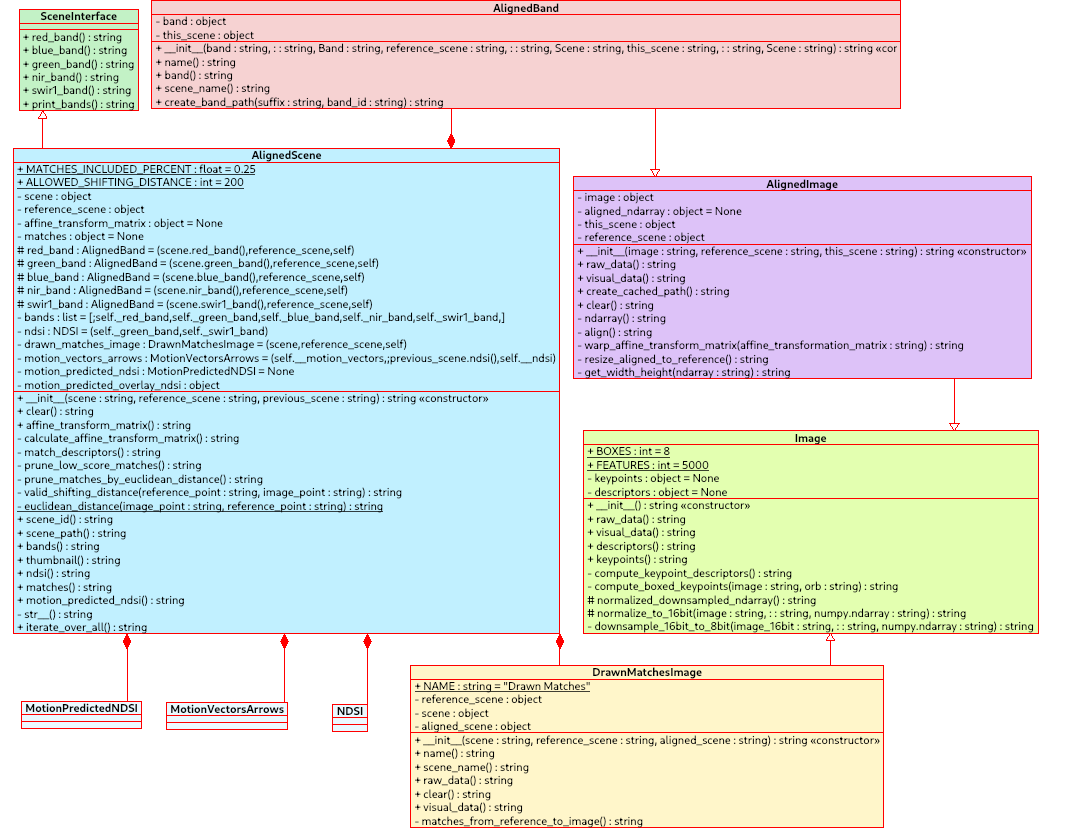
\includegraphics[scale=0.45]{../images/alignment_diagram.png}
		\caption{Technical diagram for the SceneInterface, AlignedScene, AlignedBand and Image classes.}
		\label{fig:alignment_diagram}
	\end{figure}

	%========================================================================================
	
	\subsection{Normalized Snow Difference Index}
	\label{seq:ndsi_implementation}

	The NDSI is generated by using the Formula~\ref{eq:ndsi_formula} described in section \ref{seq:NDSI_functional} on the green and shortwave infrared bands from a specific scene. Each band pixel is converted to \textbf{float32} in order to increase the \textbf{precision} of calculation; as each band is read as a n-dimensional array we can use numpy's optimised processing for generating the NDSI index image, since it converts the data and runs on native code rather than going through Python's interpretor. We then \textbf{filter} the generated image such that everything which is snow-free land will be -1 (\textbf{black}), but this is only applied for better visual analysis. In the background, we work with the full range of the image for better precision, which is the raw image. Figure~\ref{fig:ndsi_diagram} holds the technical diagram for the NDSI.
	\begin{figure}[h]
		\centering
		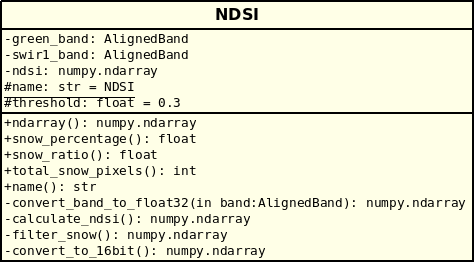
\includegraphics[scale=0.6]{../images/ndsi_diagram.png}
		\caption{Technical diagram for the NDSI class.}
		\label{fig:ndsi_diagram}
	\end{figure}

	%========================================================================================

	\subsection{NDSI Motion Matrix}
	\label{seq:motion_matrix_implementation}
	
	%========================================================================================

	\subsection{Motion Generated NDSI}
	\label{seq:motion_ndsi_implementation}
	
	\tableofcontents{}
	\addcontentsline{toc}{chapter}{List Of Figures}
	\listoffigures{}
	\addcontentsline{toc}{chapter}{List Of Tables}
	\listoftables{}
	
	\bibliographystyle{alpha}
	\bibliography{references}
		
	\chapter{Glossary}
	
	% ==================================================================
	
	\section{Acronyms}
	
		\begin{table} [H]
		\centering
		\begin{tabular} {|  l | L{10cm} |}
			\hline
			WGI & World Glacier Inventory \\ [0.2ex]
			\hline
			NDSI & Normalized Snow Difference Index \\ [0.2ex]
			\hline
			\hline
			CSV & Comma separated values \\ [0.2ex]
			\hline
			\hline
			JSON & JavaScript Object Notation \\ [0.2ex]
			\hline
		\end{tabular}
		\caption{Acronyms table }
		\label{table:acron}
	\end{table}
	\end{document}
